{\color{gray}\hrule}
\begin{center}
\section{Pipeline and Implementation Details}
%\textbf{bla bla }
\end{center}
{\color{gray}\hrule}


\subsection{General approach}

As depicted in the figure \ref{fig:general_pipeline}, our system will be subdivided into different modules each one designed to solve a specific step of the process:
\begin{itemize}[noitemsep]
\item Pre-processing: this module handles all which regards the image enhancement (denoising, light adjustement, etc...) and performs the background removal task;
\item Person Representation: this module performs pose estimation and the semantic segmentation of the person into their body parts;
\item Warping module: this module implements a geometric transformation that warps the fabric of the clothing item depending of the body shape and pose of the subject;
\item Try-On: this module generates a new image by composing the warped garment over the subject and should ensure the satisfaction of the requirements stated in the introduction section;
\item Image Retrieval: this module perform a content-based retrieval of the in-shop clothes, given a reference image.
\item Super-Resolution with Stable Diffusion: this module performs a zero-shot upscaling of the generated image of the Try-On module, based on the ControlNet architecture and some textual prompts.
\end{itemize}

Considering the e-commerce use case, during the inference, the customer inputs the target person image and the desired cloth image. The system selects the most similar in-shop cloth and then performs the virtual-try-on using these selected clothes.

\begin{figure*}[h]
\centering
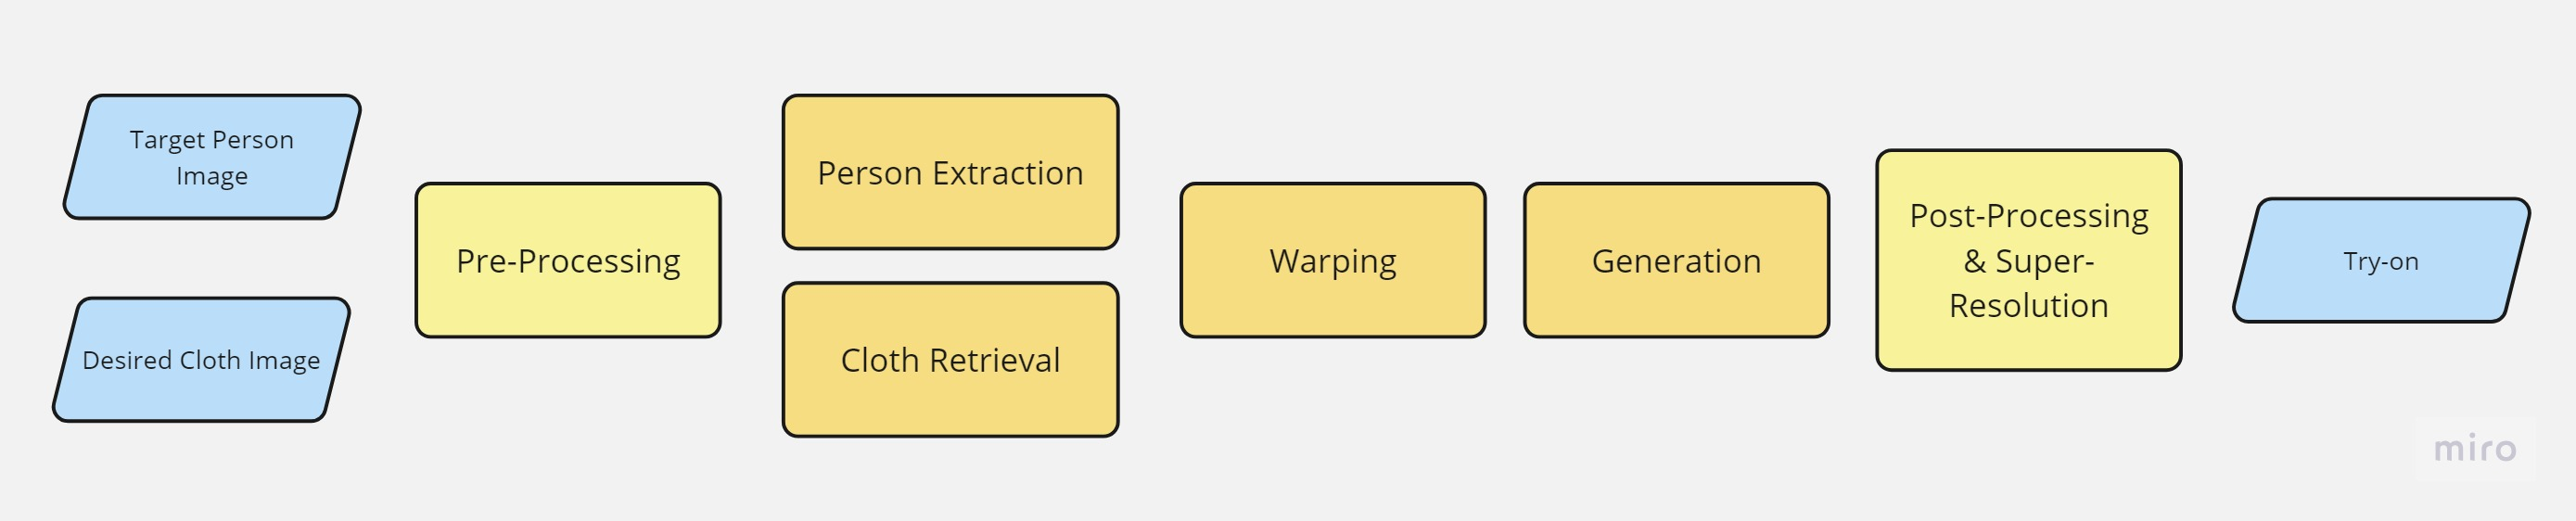
\includegraphics[width=\linewidth,height=100mm,keepaspectratio]{general_pipeline}
\caption{Overview of the pipeline}
\label{fig:general_pipeline}
\end{figure*}



In order to get across the inner workings of each module we will separate this section into subsections related to each one.


\subsection{Image Pre-Processing}
The system expects to receive two images: target person, desired cloth (it can be worn by a person or it can be cloth-only image). As the objective of the system is to be adaptable to dirty and noisy input images (so called "in-the-wild"), great care should be taken to clean such inputs.

\emph{Image Enhancing}
As the objective of the system is to be adaptable to dirty and noisy input images, in the pre-processing phase great care should be taken to clean such inputs. As such the pre-processing module applies different methods of input refinement in sequence.

Firstly the image goes through a light adjustment procedure which entails contrast stretching; then it goes through a denoising pass performed utilizing the bilateral filter.

% ??? Inserire immagini per risultato del pre-processing


\emph{Background Removal}
Given a person segmentation mask obtained by other means we perform background removal creating an rgba image and using the alpha channel and the mask to obtain only the foreground person.

% ??? inserire core del codice che esegue l'extraction
% ??? inserire spiegazione del codice



% ??? inserire citazioni necessarie



\subsection{Person Representation}
This module performs pose estimation and the semantic segmentation of the person into their body parts. It is foundamental that the person representation is cloth-agnostic: the try-on task has to preserve the target person's information (face, hair, body shape and pose), while ignoring the worn cloth. We followed the CP-VTON \citep{CP-VTON} approach, so the person representation contains three components:

\begin{itemize}[noitemsep]
\item Pose Heatmap: the pose estimation contains information about the person pose. It follows the keypoints representation in OpenPose format. From the keypoints list, it is computed an 18-channel feature map with each channel corresponding to one human pose keypoint, drawn as an $11 \times 11$ white rectangle;

\item Body Shape: a 1-channel feature map of a blurred binary mask roughly covering different parts of human body;

\item Reserved Regions: an RGB image that contains the reserved regions that are not involved in the try-on phase (for instance feet, face, hair), detected using SCHP \cite{li2019selfcorrection} that generates the segmentation mask representing the human parsing of model body parts and clothing items. There is a sligthly difference between the reserved region of the warping module and generative module and 
\end{itemize}


% ??? controllare il numero di canali
These feature maps are all scaled to a fixed resolution and concatenated together to form the cloth-agnostic person representation map $p$ of $k$ channels, where $k = 18 + 1 + 3 = 22$.
In CP-VTON, the resolution adopted is $256 \times 192$, instead we used $512 \times 384$.



\subsection{Cloth Retrieval}

The goal of this module is to match a real-world example of a garment item to the same or similar item in an online shop. We take inspiration from Exact-Street-to-Shop approach that makes two interesing points:
\begin{itemize}
	\item mixing up the geometric/perceptual and the deep-learning works pretty well;
	\item tackle the cloth-matching problem as a binary classification (match or not).
\end{itemize}

\todo{inserire immagine}
As depicted in the figure.., we built a reference repository of in-shop cloth items, using the cloth-only images in DressCode. For each cloth item we extract a new feature representation following these steps:
\begin{outline}
 \1 for each image channel (DressCode images are in the RGB format):
   \2 run ORB algorithm to compute the keypoints and the corresponding descriptors;
   \2 compute the histogram on the 256 different color levels;
   \2 concatenate all the values in a 1D tensor;
 \1 concatenate all the channel tensors in a 1D tensor and save it.
\end{outline}

The noise-clean desidered cloth image is fed to a sub-module that detects the cloth area (as a bounding box), using SCHP. From this area is extracted a new feature representation (query-feature) following the same steps presented for the cloth-only images. Then, the comparisons are performed:
\begin{outline}
\1 for each in-shop cloth:
	\2 concatenate the query-feature with the in-shop cloth feature in a 1D tensor;
	\2 fed the tensor to the deep neural network;
\1 sort and select the $k$-best matched in-shop clothes according to the matching-score given by the network. 
\end{outline}
\todo{inserire l'immagine della rete}
As depicted in the figure..., the deep neural network we designed is composed by a sequence of Fully-Connected and Normalization layers, that outputs two numbers representing, after softmax normalization, the probability of no-matching and the probability of matching. The higher one is considered the final classification result.

\todo{sistemare la formula}
To train this network, we used the regularized cross-entropy loss:
\begin{equation}
L(\theta) = \lambda_1 \cdot L_1(c_{warped}, I_{c_t}) + \lambda_{reg} \cdot L_{reg} .
\end{equation}

\todo{in Experiments, accennare al dropout}
During training, the network tried to classify both positive examples (the paired couples of worn-cloth and cloth taken) and negative examples (not paired couples). Since the number of potential negative examples was far more the number of positive examples, we used data augmentation to creating synthetic positive examples from existing one: we applyed gaussian noise to the feature representations.


\subsection{Baseline Architecture Data-Preprocessing and Data-Loading Adaptation}
% ??? mettere link all'indiano
In orderd to perform the virtual-try-on task we were inspired by CP-VTON+ \cite{CP-VTON+} public repository, but it was deprecated. Thankfully, we found a fixed and updated version.

Once we checked the proper functioning of the architecture on the VITON dataset we had to adapt the process of dataloading because the Dresscode dataset was different:
\begin{itemize}
\item it lacked binary cloth masks and binary person masks;
\item the body parts segmentation on which the module was trained used different labeling technique: the body parts were mapped in different classes
\item 
\end{itemize}

Firstly the folder structure was different, it lacked binary cloth masks and binary person masks, the body parts segmentation was performed in a total diffrent way and was not compatible and the keypoints json structure



\subsection{Warping}
% ??? inserire citazione: vedi [33] di Dress-Code
We follow the warping module proposed in CP-VTON+ \cite{CP-VTON+}.
This module transforms the input try-on garment $c$ into a warped image of the same item that matches the body pose $p$ and shape $m$. As warping function we use a thin-plate spline (TPS) geometric transformation, which is commonly used in virtual
try-on models \textit{qua va la cit.33}.  Inside this module, we aim to learn the correspondence between the inputs $(c, p, m)$ and the set of parameters $\theta$ to be used in the TPS transformation. Intuitively, the TPS fits a surface (try-on garmet) through points (feature regression output points) minimizing an energy function. Formally, it is a poli-harmonic spline function which maps a set of points $(x,y)$ on their correspondences $(x',y')$ sampled from input images. Under these terms, the warping module aims to learn how to perform such transformation.

% ??? inserire uno schema del modulo di warping
As depicted in figure blabla, the module extracts an encoded representation of the try-on garment $c$ and an encoded representation of the person representation through two separate convolutional networks.
Then, it is computed a correlation map between these representations.
This correlation map is used to predict the spatial transformation parameters $\theta$ corresponding to the $(x,y)$-coordinate offsets of TPS anchor points. 

To train this network, we used the following loss:
% ??? sostituire \times con il puntino della moltimiplicazione
% ??? L_reg nel paper mi lascia molto molto confuso
\begin{equation}
L(\theta) = \lambda_1 \cdot L_1(c_{warped}, I_{c_t}) + \lambda_{reg} \cdot L_{reg} ;
\end{equation} 
\begin{equation}
L_{reg}(G_x, G_y) = \sum{i}{i}\sum{i}{i}\sum{i}{i}i ;
\end{equation}

% ??? non mi è del tutto chiaro il significato teorico della grid regularization loss
where $L_1$ indicates the pixel-wise $L_1$-loss between the warped result $c_{warped}$ and the ground truth $c_t$. $L_{reg}$ indicates the grid regularization loss.


\subsection{Generation}
% ??? non so se questa sezione si possa considerare completa o va aggiunto altro

% ??? non sono del tutto soddisfatto della seconda metà del paragrafo
This module aims at fitting the warped garment on the target person. Previous works like CP-VTON and CP-VTON+ directly concatenate the person image $p$, the warped clothing image
$\hat{c}$, and the warped clothing mask image $\hat{cm}$ . Then the concatenated input is sent to a UNet \cite{u-net} to generate a composition mask $M_o$ and a rendered person image $I_R$. The main limitation of this approach is the inability of the convolution operator to model global long-range dependences. For this reason, we follow the CIT \cite{CIT} approach that leverage the Transfomer-based architecture and cross-modal attention mechanism that are able to capture the dependence among these three input images.

As shown in the figure \ref{fig:cit_architecture}, the three inputs goes through the patch embedding, for making the image data compatible.  Then each goes through a 1D temporal convolution to ensure the relation modeling of each element with its neighbor elements. Then the Interactive-Transformer II is utilized for modeling the global long-range correlation. The output $X_{out-II}$ of Interactive Transformer II is obtained after a linear projection and a reshape operation. Then $X_{out-II}$ is utilized for two proposes; one is to activate the important region of the overall input by adding $X_{out-II}$ to $I(p,\hat{c},\hat{cm})$; another is to guide the final mask composition as follows:

\begin{equation}
  \begin{aligned}
    I_{R}^{global} = sigmoid(X_{out-II}) \times I_R, \\
I_o = M_o \times \hat{c} + (1 - M_o) \times I_{R}^{global}
  \end{aligned}
\end{equation}

where $\times$ represents the element-wise multiplication and $sigmod$ indicates the sigmoid activation function.

\FloatBarrier
\begin{figure}
\centering
\begin{subfigure}{0.7\linewidth}
  \centering
  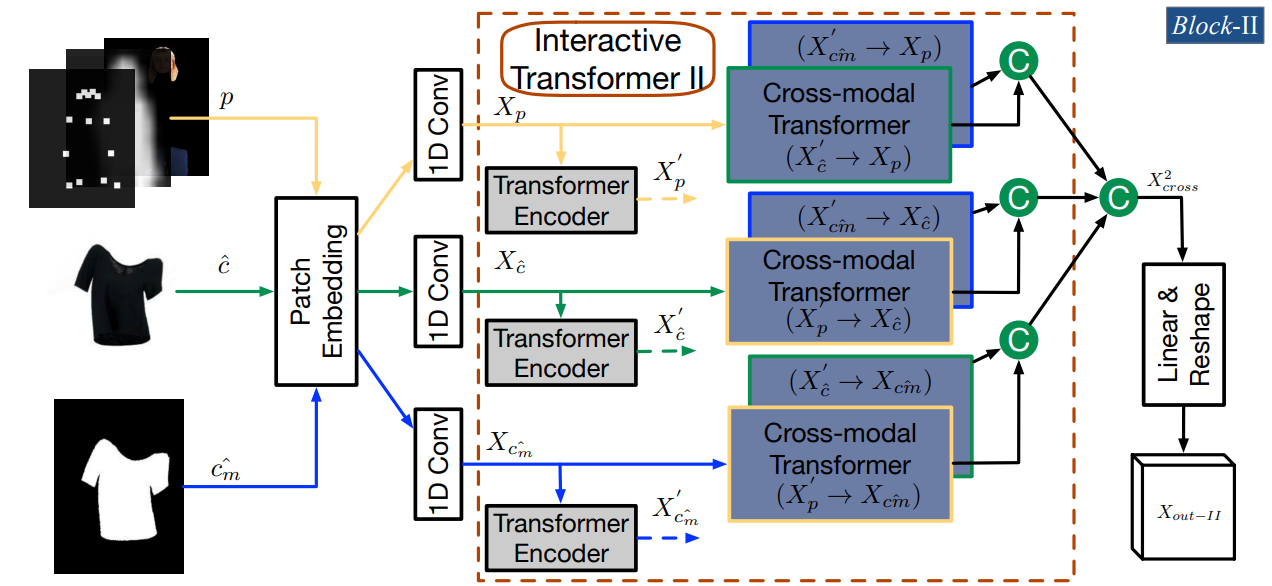
\includegraphics[width=1\linewidth]{cit_reasoning_block}
  %\caption{CIT Reasoning Block architecture, also called Interactive-Transformer II}
  \label{fig:sub1}
\end{subfigure}%
\begin{subfigure}{0.3\linewidth}
  \centering
  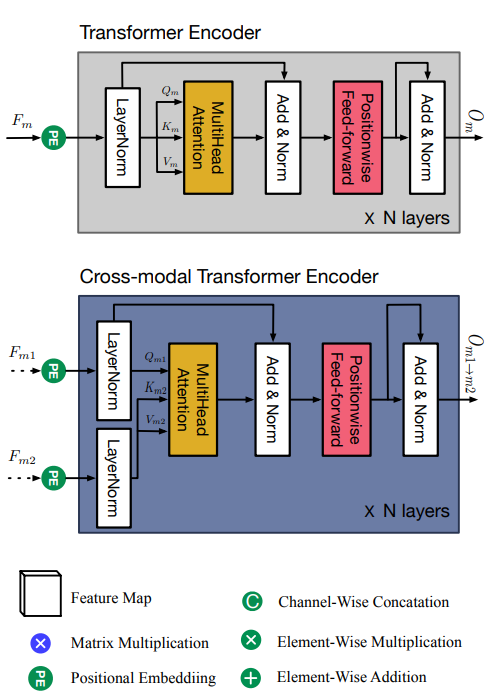
\includegraphics[width=1\linewidth]{cit_reasoning_block_2}
  %\caption{Legend}
  \label{fig:sub2}
\end{subfigure}
\caption{On the left: CIT Reasoning Block architecture, also called Interactive-Transformer II. On the right: the Transformer Encoder and Cross-Modal Transformer Encoder architetures and a legend of symbols.}
\label{fig:cit_architecture}
\end{figure}
\FloatBarrier


\subsection{Post-Processing and Super-Resolution}
